\section{ SR0005GB23 }


\subsection{Meta}

    \textbf{Title:}
    Fractured systems: a literature review of OR/MS methods applied to orthopaedic care settings and treatments

    \begin{table}[H]
        \centering
        \begin{tabular}{|c|c|c|c|c|c|c|c|c|}
            \hline
                \textbf{Rank} & \textbf{Grasp} & \textbf{Grade} & \textbf{Type} & \textbf{Outcome} & \textbf{Domain} & \textbf{COV19} & \textbf{CoI} & \textbf{DB} \\
            \hline
                4 & 87\% & A & A & P & B & Yes & No & No \\
            \hline
        \end{tabular}
        \caption{Reference's metadata}
        \label{tab:SR0005GB23}
    \end{table}

\subsection{Summary}
    Matthew et al. presented the first quantitative taxonomise review of the Operation Research and Management Sciences for Orthopaedic care services. One of the motivations for the review compilation is the ageing of the world's population, meaning more and more people will require special care. The authors searched resources in the Scopus database and produced the selection process and additional rounds of the search (back search). The authors searched by six categories in 2021 from Clarivate Jornal Citation. To analyse the extracted papers, the studies were classified by location, funding status, care area, injury location, JCR categories, implementation stage, research aims, and solution approach. The compelling visualisation of the data was shown to support the arguments. Finally, the need for further research was stated, and the limitations of the current literature review were highlighted.
    

\subsection{Notes}
    \begin{itemize}
        \item Focus on the rate of people in the world aged above 60 years.
        \item Has advanced searching techniques (pp7-8)
        \item The second work which mentions Medical Subject Headnings (MeSH)
        \item Six categories in the 2021 Clarivate Jornal Citation Report (JCR)
    \end{itemize}


\subsection{Reading}

    \textbf{Abstract:}
    The healthcare management is challanged with Earth growing population size and consequences of the COVID-19 pandemic. This literature review conducts a structurate overview of 492 publications in the field of Operational Research and Management Science applications. The authords of the review found a research gap and addressed it in the work.
    
    \textbf{Objectives / 1st page:}
    The aim is to quantify and taxonomise the current state of the OR/MS approaches implemented in orthopadic department.
    
    \textbf{Page 2:}
    There have not been direct guidances how OR/MS applied in the practice to optimise ortophedic departments prior to this review. Matthew Howells et al. \cite{x122} summarised some other literature reviews and concluded that for the best of their knowlesge there are no literature review on OR/MS from the perspective of orthopedic health care services.
    
    \textbf{Page 3:}
    The reviewd papers are classified into three contexts: general, medical, and methodological. The studies for review were searched accross 6 categories to have diverse perspective on the OR/MS:

    \begin{itemize}
        \item Health Case Sciences \& Services (HCSS);
        \item Health Policy and Services (HPS);
        \item Industrial Engineering (IE);
        \item Medical Informatics (MI);
        \item Operations Research and Management Sciences (OR/MS);
        \item Orthopedic (T\&O);
    \end{itemize}

    The authors also define three types of data sources:

    \begin{itemize}
        \item Primary data - collected by researchers themselfs;
        \item Secondary data - collected by third parties and used by researchers;
        \item Expert opinion - generalisations on the public research with no direct access to the research data;
    \end{itemize}

    \begin{figure}[H]
        \centering
        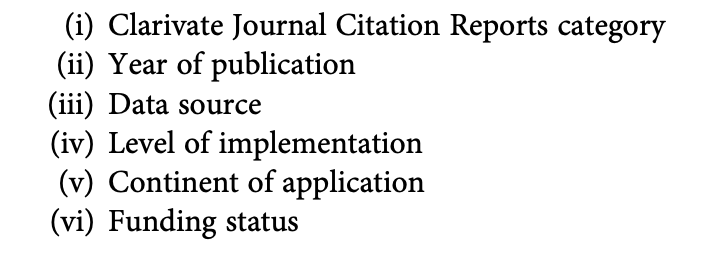
\includegraphics[width=.8\textwidth]{figures/SR0005GB23/fig1.png}
        \caption{List of data extracted from the reviewed studies in \cite{x122}.}
        \label{fig1:SR0005GB23}
    \end{figure}
    
    \textbf{Page 4:}
    The research implementation is categorised into theoretical, conseptualised, and implemented works. The origin and the funding status of the reviewead research are included in the scope of this work. The orthopeci healthcare services are segmented on the smaller groups defined by the type of the illness by longtitude and the bodybart it effected.
    
    \textbf{Page 5:}
    On this page the authors dive into more segmentations and classifications of the studies by the type of caregiver and environment (primary, secondary, tertiary, community, patient progression), by hospitalisation type (assignment, inpatients, surgery, post-surgery, rehabilitaion, follow-up) and by scope (clinical, department, or hospital). 
   
    \textbf{Page 6:}
    Further classtering of the research is defined by the healthcare funding providar (patient, provider, societal), by research aims (evaluation, forecasting, improvement), by algorithms applyed (Decision Analysis, Graph Theory, Heuristics, Markov, Multi-Critaria Decision-Making (MCDM), Optimisation, Queueing Theory, Soft OR, Statistical Analysis). The last classification is not not exclusive the approach can be both the delphy algorithm and an optimisation.
    
    \textbf{Page 7:}
    There are three more approches of the OR/MS research grouping: by outcomes (cost, health, time), by functional area (Bed Management, Capacity Planning, Cost Analysis, Cost-Effectivenes Analysis, Cost-Utility Analysis, Expected-Valye Decision Analysis, Health-Unity Analysis, Location Planning, Manufacturing, Medical Decisions, Medical Simulations, Patient Scheduling, Risk-Benefit Analysis, Staff Utilisation, and System Design and Planning), and by planning decision levels (strategic, tactical, and operational which is futher segmented into offline and online scheduling). 
    For searching the publications the Scopus database was used. The Appendicies A an B shows the searching terms and requests.
    
    \textbf{Page 8:}
    This page present an advanced searching techniques and the proces of screening the 1,936 paper to 14.88\% for the full text review and 2.14\% in the final analysis. 
    
    \textbf{Page 9:}
    Here the authors explain the next steps for literature search such as back search using works in the initial search (Appendix C).
    \begin{figure}[H]
        \centering
        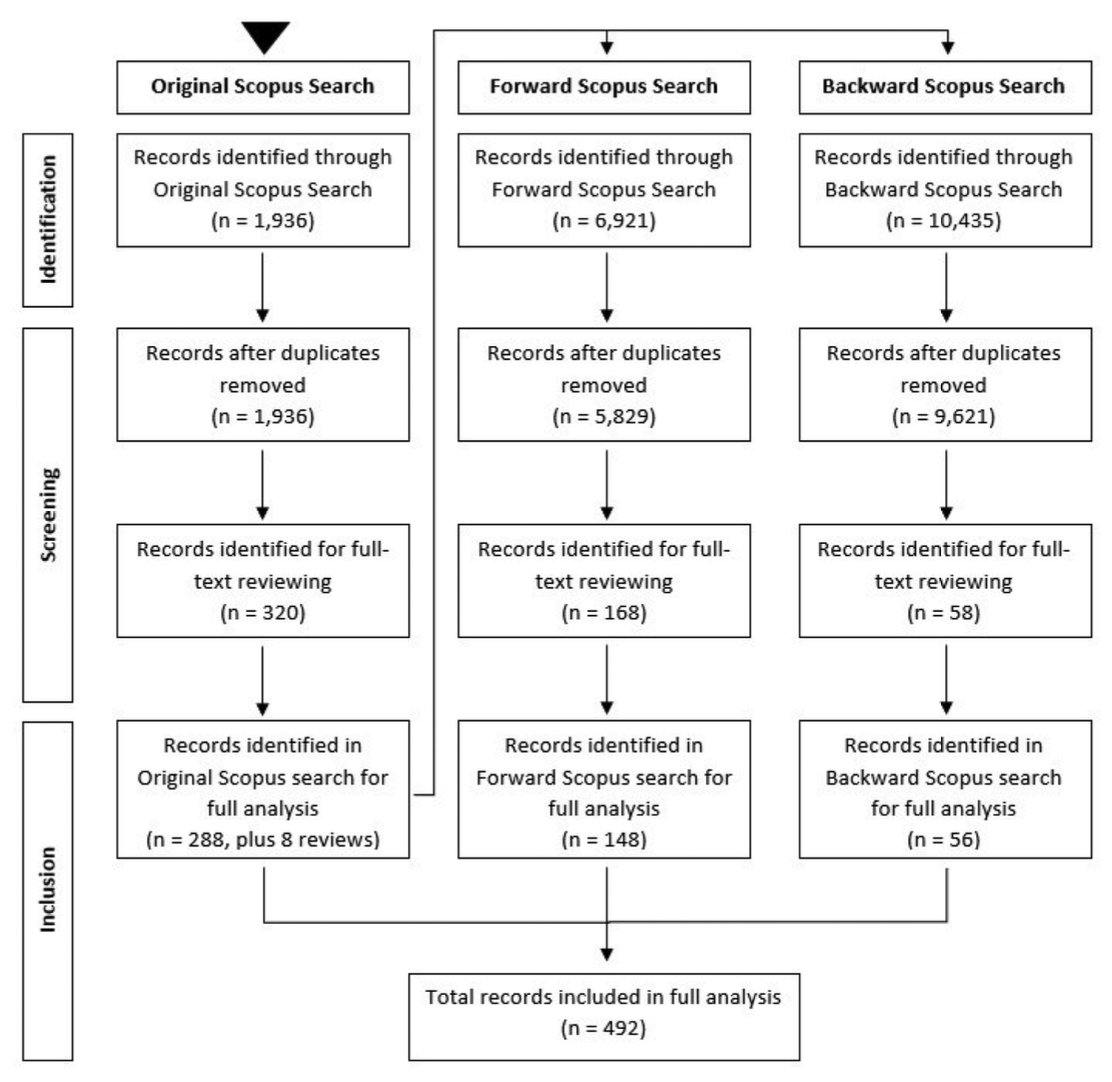
\includegraphics[width=.8\textwidth]{figures/SR0005GB23/fig2.png}
        \caption{Flow diagram of the literature search in \cite{x122}.}
        \label{fig2:SR0005GB23}
    \end{figure}
    
    \textbf{Page 10:}
    The authors answare questions Who, When, and Under which surcumstances the model was developed and published.
    
    \textbf{Page 11:}
    Literature analysis by the search type and the funding.
    \begin{figure}[H]
        \centering
        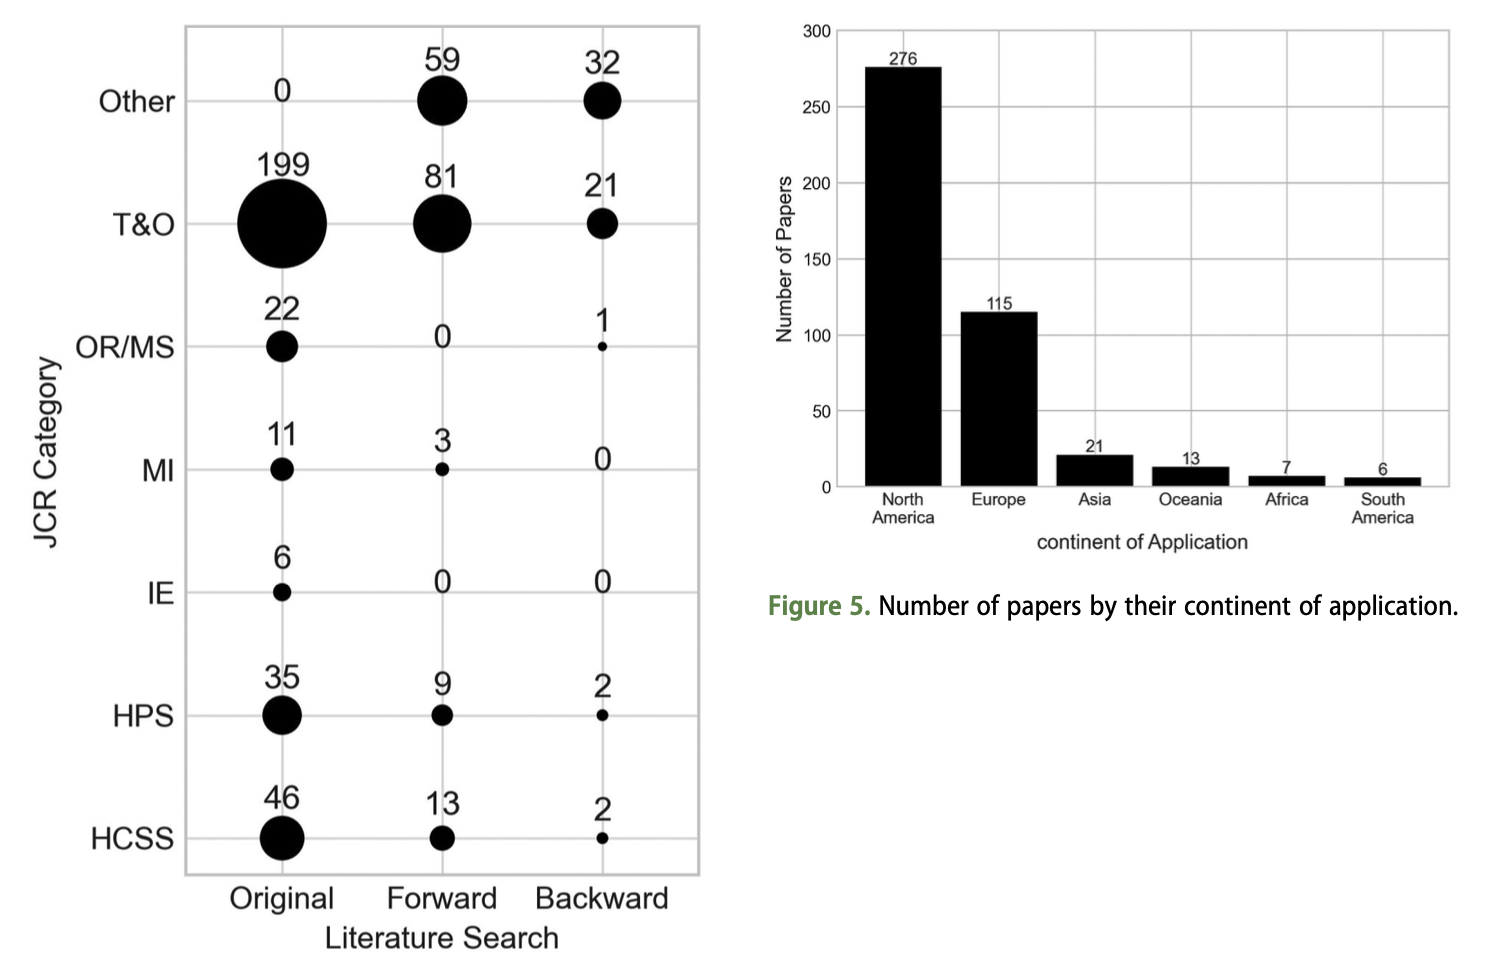
\includegraphics[width=.8\textwidth]{figures/SR0005GB23/fig3.png}
        \caption{Literature search analysis in \cite{x122}.}
        \label{fig3:SR0005GB23}
    \end{figure}

    \textbf{Page 12:}
    On this page the analysis of the papers by groups mentioned earlier.
    
    \textbf{Page 13:}
    In this part there are more quantitative analysis of studies by care area and number of secondaty/tertiary pathways.
    
    \textbf{Page 14:}
    Here the thoughts and answares to why the computational methods for orthopedic techniques have been developed.
    \begin{figure}[H]
        \centering
        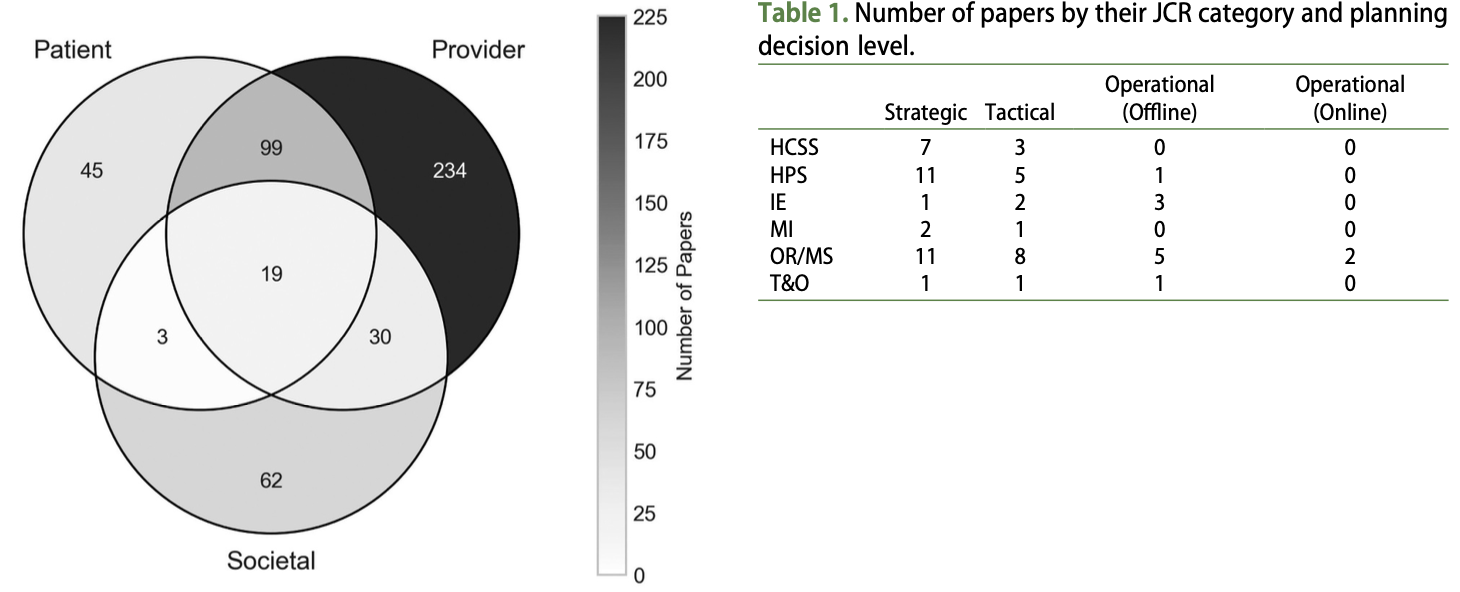
\includegraphics[width=1\textwidth]{figures/SR0005GB23/fig4.png}
        \caption{Fundings and JCR category analysis in \cite{x122}.}
        \label{fig4:SR0005GB23}
    \end{figure}

    \textbf{Page 15:}
    The authors analysethe papers research aims, research outcomes, and number of papers with the real world implementation (which is less then 5\%).

    \textbf{Page 16:}
    The count of papers in each group by data type was analysed in this part of the review. 
    \begin{figure}[H]
        \centering
        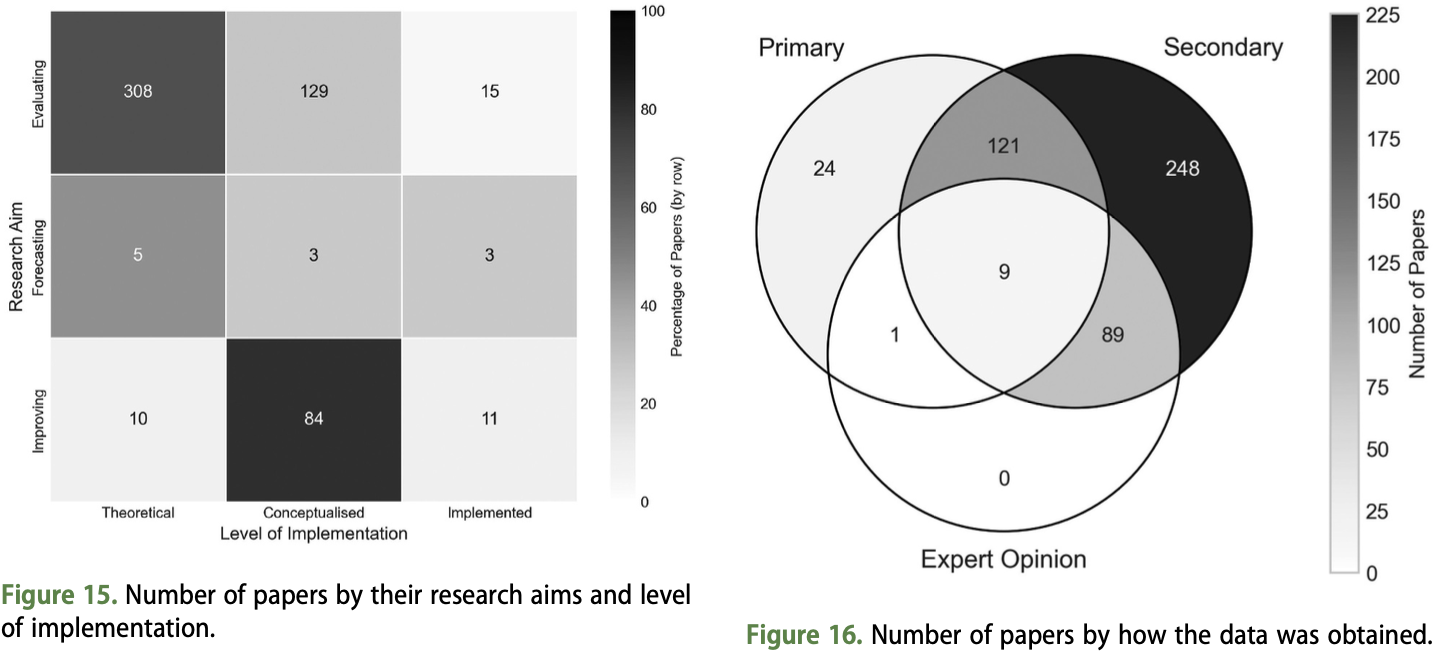
\includegraphics[width=1\textwidth]{figures/SR0005GB23/fig5.png}
        \caption{Research aim-implementation chart and types of used data chart in \cite{x122}.}
        \label{fig5:SR0005GB23}
    \end{figure}

    \textbf{Page 17:}
    On this page the developed aproaches have been quantified by number of papers.
    
    \textbf{Page 18:}
    \begin{figure}[H]
        \centering
        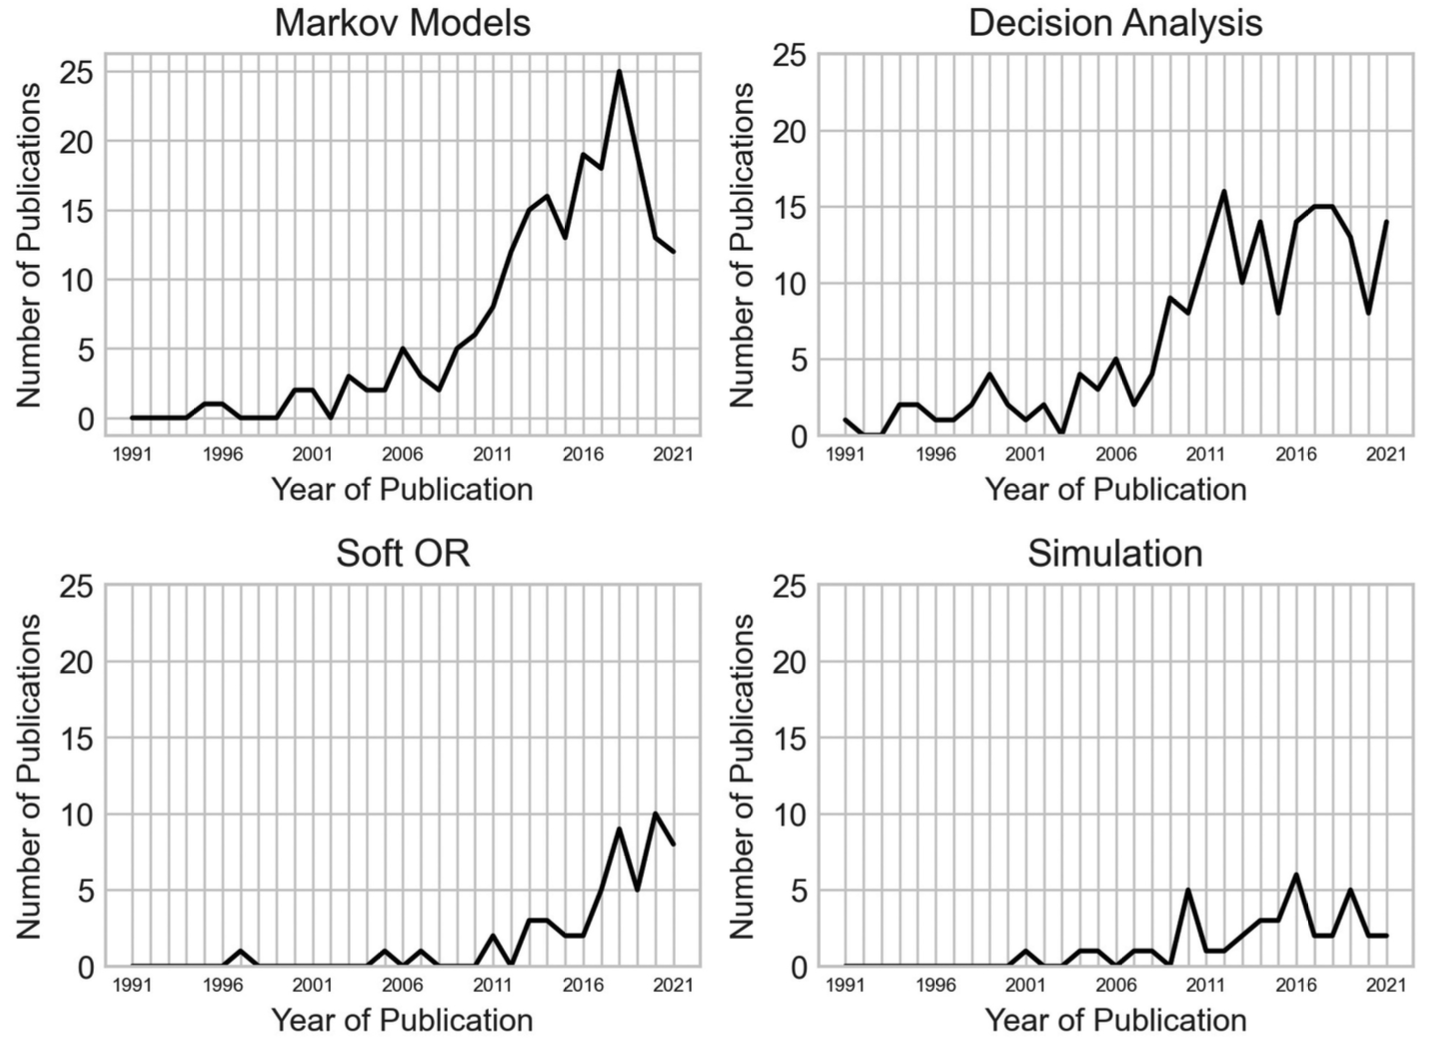
\includegraphics[width=.9\textwidth]{figures/SR0005GB23/fig6.png}
        \caption{Trends from 1991 to 2021 from \cite{x122}.}
        \label{fig6:SR0005GB23}
    \end{figure}
    
    \textbf{Page 19:}
    \begin{figure}[H]
        \centering
        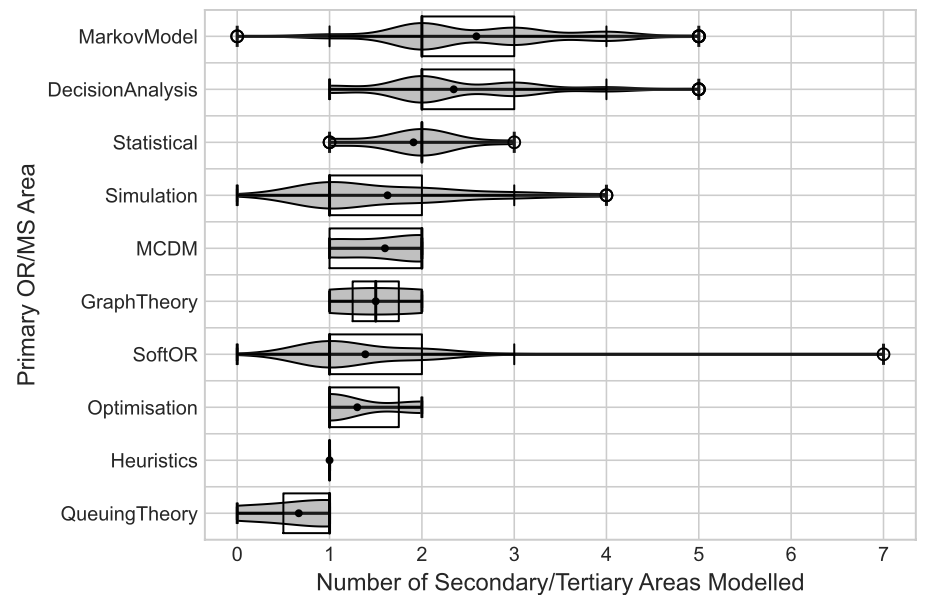
\includegraphics[width=.9\textwidth]{figures/SR0005GB23/fig7.png}
        \caption{Number of papers by their primary OR/MS method area and level of implementation from \cite{x122}.}
        \label{fig7:SR0005GB23}
    \end{figure}
    \begin{figure}[H]
        \centering
        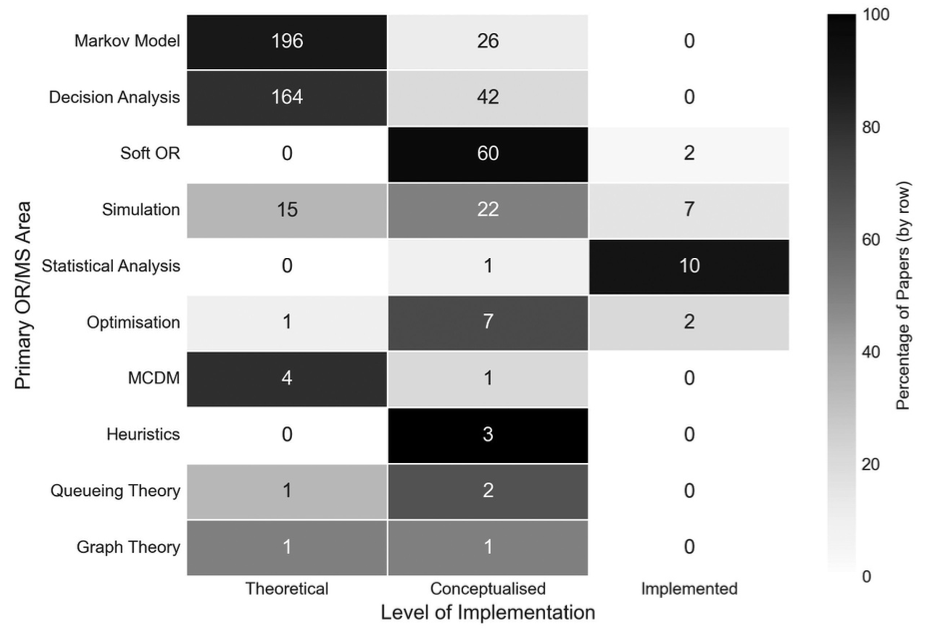
\includegraphics[width=1\textwidth]{figures/SR0005GB23/fig8.png}
        \caption{Distribution of the number of secondary/tertiary care areas modelled by each primary or area from \cite{x122}.}
        \label{fig8:SR0005GB23}
    \end{figure}

    \textbf{Page 20:}
    Here the authors focus on the different type of simulations and their efficiency. Next the discussion on the work is introduces and the authors hihglighted the limitations of the work in using just Scopus database with no concern to Medline and PubMed databases.

    \textbf{Page 21:}
    The authors organise the materials in CSV filem Jupyter Notebook and Zenodo for research replicability. Next there are reflections on the frequency of the OR/MS research in the different regions of the world and on the trends in different categories.

    \textbf{Page 22:}
    At the start of this page the non-resultive search and some drawbacks were discussed.

    \textbf{Conclusion:}
    Matthew et al. summariese the current review in further points: the whole pathway modeling, capacity planning, optimisation, simulation, and queueing theories, mix-methodology, model implementation, addressing population ageing issue. These points are directions requiring further research.